\documentclass[12pt,a4paper]{report}

\usepackage{alltt, fancyvrb, url}
\usepackage{graphicx}
\usepackage[utf8]{inputenc}
\usepackage{float}
\usepackage{xcolor}
\usepackage{hyperref}
\usepackage{longtable}

\usepackage{enumitem}
\usepackage{amsmath}
\usepackage{geometry}
\geometry{margin=1in}

\usepackage{newlfont}
\usepackage{gensymb}

\usepackage[italian]{babel}
\usepackage[italian]{cleveref}

\graphicspath{ {./src/img} }

\textwidth=450pt\oddsidemargin=0pt
\begin{document}

\begin{titlepage}
\begin{center}
{{\Large{\textsc{Alma Mater Studiorum $\cdot$ Università di Bologna}}}} \rule[0.1cm]{15.8cm}{0.1mm}
\rule[0.5cm]{15.8cm}{0.6mm}
{\small{\bf CORSO DI LAUREA IN INGEGNERIA E SCIENZE INFORMATICHE \\ A.A. 2024/25 }}
\end{center}
\vspace{15mm}
\begin{center}
{\LARGE{\bf Smart City - Mobilità Integrata}}
\end{center}
\begin{center}
{\LARGE Relazione per il corso di Basi di Dati }
\end{center}

\vspace{8mm}
\begin{center}
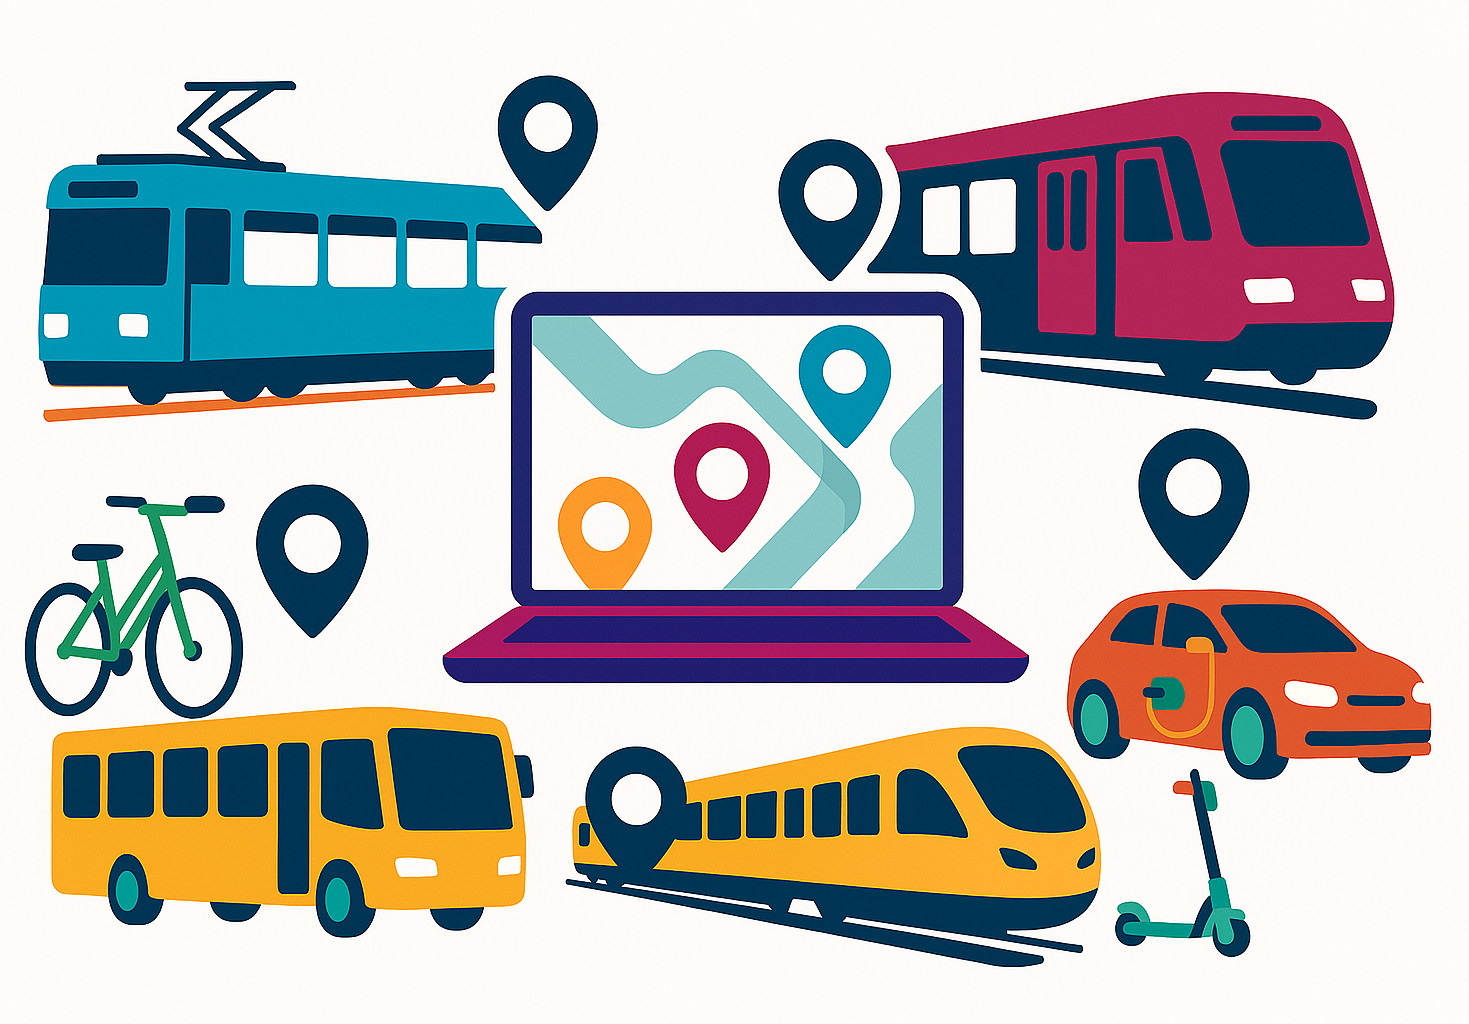
\includegraphics[width=0.8\textwidth]{Copertina}
\end{center}
\vspace{10mm}

{\large{\bf \noindent
Componenti del gruppo nr.2743:\\}
Bartocetti Enrico, matr. 0001115097\\
Benedetti Nicholas, matr. 0001114021\\
Tazzieri Nicolas, matr. 0001114078}

\end{titlepage}

\tableofcontents


\chapter{Analisi dei requisiti}

\section{Intervista iniziale}
Si vuole realizzare il software per la gestione del trasporto pubblico a lungo e corto raggio.
A seguito dell’intervista è stata prodotta la seguente descrizione delle specifiche del sistema in linguaggio naturale:
\\ \\
\textit{Le città di Vergineto, Urbania e San Giovanni in Marignano si sono accordate per avviare il progetto “Smart mobility 2030”, e richiedono un software per la gestione Smart e integrata del trasporto pubblico urbano ed extraurbano.}

\textit{Il sistema dovrà gestire diversi mezzi di TPL (Trasporto Pubblico Locale), quali bus, tram, metropolitana e treni ma in futuro potrebbe sorgere la necessità di aggiungerne di nuovi (ad esempio in seguito alla creazione di linee per i filobus). Ogni mezzo potrà percorrere diverse linee: ciò significa che un autobus utilizzato oggi per la linea 15, domani potrà percorrere la linea 21.}

\textit{Per ogni linea verranno effettuate delle fermate a orari prestabiliti. Potranno essere create anche linee straordinarie, ad esempio delle navette per eventi cittadini, di cui dovranno essere specificati periodo di validità, orari e fermate.}

\textit{Inoltre, per ridurre l’inquinamento nelle nostre città, verranno creati degli spazi riservati per lo sharing di biciclette, scooter e biciclette, e verranno aggiunte delle colonnine per la ricarica elettrica in modo da incentivare sia l’acquisto di auto elettriche sia l’utilizzo di monopattini o bici elettriche.}

\textit{Sarà disponibile una piattaforma online, nella quale si potranno visualizzare le diverse linee e le fermate che i mezzi effettuano con i relativi orari, nonché la disponibilità di posti liberi nelle aree di bikesharing e nelle colonnine elettriche. È anche prevista la registrazione di utenti “cittadini”, che potranno acquistare biglietti e abbonamenti. }

\textit{Un unico biglietto vale per tutti i mezzi di trasporto, e si vuole memorizzarne la durata, la data di convalida, la data di acquisto ed il titolare nel caso venga acquistato online: infatti un biglietto potrà anche essere acquistato da un fornitore fisico (ad esempio le tabaccherie della città). Sono presenti diverse tipologie di biglietti che differiscono in base alla durata dalla convalida e al prezzo. Gli abbonamenti sono biglietti che hanno una durata superiore ad un giorno.}

\textit{Si richiede anche la gestione dei dipendenti. In particolare, dovranno essere gestiti diversi autisti a cui verranno assegnati diversi mezzi in diversi slot orari. Sono inoltre presenti i controllori: in certi orari dovranno controllare diverse linee e saranno in grado di emettere multe. Gli orari e le linee da controllare vengono stabilite dal gestore delle linee di trasporto: ad esempio verranno prese in particolare considerazione quelle dove non ci sono molti incassi, ovvero dove è ipotizzabile una maggior evasione tariffaria, generando ingenti perdite economiche. Infine, l’amministratore del sistema potrà registrarsi in un portale specifico nel quale potrà gestire autisti, controllori e le linee. Inoltre, avrà la possibilità di visualizzare diverse statistiche riguardanti il sistema di trasporto, con enfasi particolare nei ricavi dei biglietti e nel tasso di evasione.}

\textit{Dovranno essere gestiti i lavori di manutenzione relativi a linee e mezzi per cui saranno specificati gli eventuali enti privati che li svolgeranno. Per le manutenzioni sarà richiesto di specificare una data di inizio e fine lavori, ed eventuali variazioni di servizio dovranno essere visualizzate al pubblico.}


\section{Prima fase di analisi}
Nell’analisi dell’intervista effettuata tempo addietro, abbiamo notato che il committente non è stato abbastanza esaustivo su alcuni argomenti.
Si è quindi resa necessaria un’ulteriore intervista per comprendere meglio il funzionamento di:
\begin{itemize}
	\item Sistema di acquisto e convalida di biglietti
	\item Gestione degli spazi speciali
	\item Gestione delle multe
\end{itemize}
\noindent Riportiamo le risposte R alle varie domande D.

\paragraph{D:}
“Come devono essere gestiti i biglietti, dal loro acquisto fino alla convalida?”
\\ {\bf R:} “I biglietti possono essere acquistati tramite il sito web, le biglietterie fisiche (sia dell’azienda sia da altri venditori autorizzati) e ticketmachine.
Ogni mezzo sarà dotato di una obliteratrice che, comunicando con il sistema informativo, alla lettura di un biglietto (tramite codice a barre stampato sul biglietto fisico o letto dal proprio dispositivo) ne controlla la validità e in caso affermativo lo registra come convalidato.”

\paragraph{D:}
“Cosa deve essere mostrato riguardo agli spazi per la mobilità sostenibile?”
\\ {\bf R:} “L’idea è quella di far vedere giusto una panoramica riguardo agli spazi.
In particolare, basta visualizzarne la posizione, l’indirizzo, un nome simbolico e quanti sono i posti rimanenti (quante biciclette rimanenti se si tratta di biciclette, quante colonnine se si tratta di colonnine elettriche, ecc.).
Inoltre, uno spazio può essere legato ad una fermata per rendere agevole il collegamento con aree non raggiunte dalle linee del TPL (es. appena scendo dal bus mi trovo nei pressi di una zona per il bike sharing)”

\paragraph{D:}
“Come funziona il sistema delle multe?”
\\ {\bf R:} “Le multe possono essere emesse dal personale qualificato a seguito di controlli effettuati sulle linee.
A ogni causale della multa corrisponde un certo importo base, a cui dovranno essere aggiunte eventuali penali per recidiva dell’utente o per ritardi nel pagamento.”


\section{Concetti principali}
Per rendere meglio fruibile la descrizione, abbiamo deciso di rimuovere eventuali ambiguità, seguendo la tabella qua sotto.

\begin{table}[h!]
\begin{tabular}{|l|l|}
\hline
\textbf{Termine} & \textbf{Nuovo Termine} \\
\hline
Mezzi di TPL & Mezzi di trasporto \\
Spazi riservati per il carsharing, … & Hub mobilità \\
Biglietti, Abbonamenti & Titolo di Viaggio \\
Gestore delle linee & Amministratore di Sistema \\
\hline
\end{tabular}
\end{table}

A seguito dell’intervista aggiuntiva è stata redatta la seguente descrizione del dominio in linguaggio naturale. Ambiguità e informazioni ridondanti sono state eliminate per garantire una miglior fruizione della descrizione:
\\ \\
Le città di Vergineto, Urbania e San Giovanni in Marignano si sono accordate per avviare il progetto “Smart mobility 2030”, e richiedono un software per la gestione Smart e integrata del trasporto pubblico urbano ed extraurbano.

Il sistema dovrà gestire diversi \underline{\texttt{mezzi di trasporto}}, quali \underline{\texttt{bus}}, \underline{\texttt{tram}}, \underline{\texttt{metropolitana}} e \underline{\texttt{treni}} lasciando la possibilità di aggiungerne altri in futuro. Ogni mezzo di trasporto potrà percorrere diverse \underline{\texttt{linee}}.

Una linea può essere \underline{\texttt{ordinaria}} o \underline{\texttt{straordinaria}}. Ogni linea effettua \underline{\texttt{fermate}} ad \underline{\texttt{orari}} prestabiliti. Per una linea straordinaria dovrà essere specificato il periodo di validità della linea.

Dovranno essere gestiti degli \underline{\texttt{hub mobilità}}, riservati per la ricarica elettrica e lo sharing di bici, monopattini e scooter. In particolare, si devono memorizzare la posizione, l’indirizzo, un nome simbolico e quanti sono i posti rimanenti. Inoltre, ad un hub mobilità può essere \underline{\texttt{associato}} ad una fermata.

Sarà disponibile una piattaforma online, nella quale si potranno visualizzare le diverse linee e le fermate che i mezzi effettuano con i relativi orari, nonché la disponibilità di posti liberi negli hub mobilità. È anche prevista la registrazione di \underline{\texttt{utenti cittadini}}, che potranno \underline{\texttt{acquistare}} \underline{\texttt{titoli di viaggio}}, che si dividono in \underline{\texttt{biglietti}} e \underline{\texttt{abbonamenti}}.

Un unico titolo di viaggio vale per tutti i mezzi di trasporto e vuole memorizzarne la durata, la data di convalida, la data di acquisto e l’utente cittadino associato nel caso sia un \underline{\texttt{biglietto digitale}}. Sono presenti diverse \underline{\texttt{tipologie}} di titoli di viaggio che differiscono in base alla durata dalla convalida e al prezzo. Gli abbonamenti sono biglietti che hanno una durata superiore ad un giorno. I biglietti possono essere acquistati anche in biglietterie fisiche e ticketmachine. Ogni mezzo di trasporto sarà dotato di una obliteratrice che, comunicando con il sistema informativo, alla lettura di un biglietto ne controlla la validità, e in caso affermativo, lo registra come \underline{\texttt{convalidato}}.

Si richiede anche la gestione dei \underline{\texttt{dipendenti}}. Essi si dividono in \underline{\texttt{Autisti}}, \underline{\texttt{Controllori}} e \underline{\texttt{Amministratori di sistema}}. Agli Autisti a verranno assegnati diversi mezzi di trasposto in slot orari diversi. I controllori dovranno controllare diverse linee negli slot orari assegnati, e saranno in grado di emettere \underline{\texttt{multe}}.  A ogni \underline{\texttt{causale della multa}} corrisponde un certo importo base, a cui potranno essere aggiunte eventuali penali per recidiva dell’utente o per ritardi nel pagamento. Gli orari e le linee da controllare vengono stabilite dall’amministratore di sistema. Infine, l’amministratore del sistema potrà registrarsi in un portale specifico nel quale potrà gestire autisti, controllori e le linee. Inoltre, avrà la possibilità di visualizzare diverse statistiche riguardanti il sistema di trasporto, con enfasi particolare nei ricavi dei titoli di viaggio e nel tasso di evasione.

Dovranno essere gestiti i lavori di \underline{\texttt{manutenzione}}, che possono coinvolgere \underline{\texttt{linee}} e \underline{\texttt{mezzi di trasporto}}, per cui saranno specificati gli eventuali \underline{\texttt{enti privati}} che li svolgeranno. Per le manutenzioni sarà richiesto di specificare una data di inizio e fine lavori, ed eventuali \underline{\texttt{variazioni di servizio}} che coinvolgono linee dovranno essere visualizzate al pubblico.

\chapter{Progettazione Concettuale}
\section{Schema Scheletro}
\section{Raffinamenti Proposti}
\section{Schema Concettuale Finale}

\chapter{Progettazione Logica}
\section{Stima del Volume dei Dati}
Per poter gestire al meglio il carico di lavoro della base di dati, insieme al committente si è creata una stima del volume dei dati per entità e associazioni che il database dovrà gestire, di cui se ne riportano i numeri nella Tabella \ref{table:volumeDati}.
La stima è valida per un carico di lavoro di circa 6 mesi.

\begin{longtable}{|p{7.5cm}|r|c|}
\caption{Stima del volume dei dati}
\label{table:volumeDati}\\
\hline
\textbf{NOME} & \textbf{VOLUME STIMATO} & \textbf{E/A} \\
\hline
\endhead

ABBONAMENTO & 30.000 & E \\
\hline
AMMINISTRATIVO & 10 & E \\
\hline
ATTUAZIONE CORSA & 250.000 & E \\
\hline
AUMENTO & 10 & E \\
\hline
AUTISTA & 130 & E \\
\hline
AZIENDA & 15 & E\\
\hline
BIGLIETTO DIGITALE & 150.000 & E \\
\hline
BIGLIETTO FISICO & 150.000 & E \\
\hline
CAUSALE MULTA & 10 & E \\
\hline
CONTENUTO HUB & 4 & E \\
\hline
CONTROLLORE & 40 & E \\
\hline
DIPENDENTE & 180 & E \\
\hline
FERMATA & 450 & E \\
\hline
HUB MOBILITÀ & 225 & E \\
\hline
LINEA & 75 & E \\
\hline
MANUTENZIONE & 50 & E \\
\hline
MANUTENZIONE LINEA & 10 & E \\
\hline
MANUTENZIONE MEZZO & 40 & E \\
\hline
MEZZO & 160 & E \\
\hline
MULTA & 10.000 & E \\
\hline
ORARIO LINEA & 1500 & E \\
\hline
ORDINARIA & 65 & E \\
\hline
PERSONA & 20.000 & E \\
\hline
STRAORDINARIA & 10 & E \\
\hline
TARIFFA ABBONAMENTO & 5 & E \\
\hline
TARIFFA BIGLIETTO & 10 & E \\
\hline
TIPOLOGIA MEZZO & 4 & E \\
\hline
TITOLO DI VIAGGIO & 750.000 & E \\
\hline
TRATTA & 1.000 & E \\
\hline
UTENTE & 10.000 & E \\
\hline
ACQUISTO ABBONAMENTO & 30.000 & A \\
\hline
ACQUISTO BIGLIETTO & 150.000 & A \\
\hline
ARRIVO & 1.000 & A \\
\hline
ASSUNZIONE & 160 & A \\
\hline
CONDUCENTE & 250.000 & A \\
\hline
CONTENUTO & 450 & A \\
\hline
CONTROLLO & 50.000 & A \\
\hline
CONVALIDA & 200.000 & A \\
\hline
EFFETTUAZIONE & 250.000 & A \\
\hline
EMISSIONE & 10.000 & A \\
\hline
FASCIA ABBONAMENTO & 30.000 & A \\
\hline
FASCIA BIGLIETTO & 300.000 & A \\
\hline
IMPIEGO & 250.000 & A \\
\hline
INCARICO & 25 & A \\
\hline
INCREMENTO & 10 & A \\
\hline
INTESTAZIONE & 10.000 & A \\
\hline
MODIFICA & 10 & A \\
\hline
NECESSITA & 40 & A \\
\hline
PARTENZA & 1.000 & A \\
\hline
PRESENZA & 165 & A \\
\hline
RIFERIMENTO & 10.000 & A \\
\hline
SOSTITUZIONE & 10 & A \\
\hline
SPECIFICAZIONE & 1.500 & A \\
\hline
TIPO LINEA & 75 & A \\
\hline
TIPOLOGIA & 10.000 & A \\
\hline
TRAGITTO & 1.500 & A \\
\hline
\end{longtable}


\section{Descrizione operazioni}
Riportiamo in Tabella \ref{table:operazioni} le principali operazioni che saranno svolte sulla base di dati, marcando con un asterisco (*) le operazioni di cui è necessario calcolare i costi dati da attributi ridondanti.

\begin{longtable}{|c|p{7.5cm}|c|l|l|}
\caption{Numero stimato di operazioni per settimana, con tipo di utente che le effettua}
\label{table:operazioni}\\
\hline
\textbf{\#} & \textbf{Operazione} & \textbf{Op / 7gg} & \textbf{Tipo Utente} & Nome \\
\hline
\endhead
1*  & Visualizzazione di tutte le linee attive & - & Tutti & Enr \\
\hline
2* & Visualizzazione fermate e orari di una linea & 3.500 & Tutti & Svit \\
\hline
3 & Visualizzazione degli hub mobilità & 500 & Tutti & Nick \\
\hline
4* & Visualizzazione orario e mezzo assegnato & 150 & Autista & Svit  \\
\hline
5* & Visualizzazione orario e linee assegnate & 100 & Controllore & Enr \\
\hline
6 & Estrazione delle linee con più convalide nell'ultimo mese & 3 & Amministratore & Svit  \\
\hline
7 & Estrazione delle manuntenzioni che coinvolgono un determinato mezzo & 5 & Amministratore & Enr \\
\hline
8 & Estrazione delle manuntenzioni ed eventuali linee sostitutive che coinvolgono una linea & 5 & Amministratore & Nick \\
\hline
9 & Visualizzazione incassi dati dalle convalide per una linea & 10 & Amministratore & Svit  \\
\hline
10 & Estrazione degli incassi per tipo di titolo in periodo definito & 5 & Amministratore & Enr     \\
\hline
11 & Estrazione delle linee con più multe negli ultimi 3 mesi & 2 & Amministratore  & Nick  \\
\hline
12 & Estrazione delle 5 linee con manutenzioni più gravose (in termini linee sostitutive e durata) & 2 & Amministratore  & Svit     \\
\hline
13 & Estrazione delle linee con \textgreater 5 controlli/giorno e \textless = 10 multe/giorno & 3 & Amministratore   & Nick   \\
\hline
14 & Visualizzazione delle linee con il maggior tempo di percorrenza & 2 & Amministratore & Svit  \\
\hline
15 & Estrazione delle linee con più hub mobilità lungo il percorso & 3 & Amministratore & Enr \\
\hline
16 & Media di soldi spesi in multe per persona & 2 & Amministratore & Nick \\
\hline
17 & Visualizzazione delle aziende che non hanno effettuato nessuna manutenzione nell'ultimo mese & 4 & Amministratore & Svit  \\
\hline
18 & Visualizzazione delle fermate in cui è presente un hub mobilità contenente tutti i tipi di servizi green & 1 & Amministratore  & Enr \\
\hline
19* & Inserimento di una variazione di servizio & 1 & Amministratore & Nick \\
\hline
20* & Aggiunta di una tratta a una linea esistente & 1 & Amministratore & Enr \\
\hline
21* & Creazione di una nuova linea & 1 & Amministratore & Nick \\
\hline
\end{longtable}

\section{Analisi delle operazioni}
Indichiamo con:
\begin{itemize}
	\item ${C_{tot}}$ il costo totale dell'operazione.
	\item ${O_{settimana}}$ il numero di volte che l'operazione verrà eseguita in una settimana
	\item ${A_{scrittura}}$ il numero di accessi in scrittura effettuato da un'operazione
	\item ${A_{lettura}}$ il numero di accessi in lettura effettuato da un'operazione
\end{itemize}

\noindent Di seguito eseguiamo l'analisi delle operazioni presenti in Tabella \ref{table:operazioni}, riportando lo schema di navigazione, la tabella degli accessi e il calcolo del costo della specifica operazione per ogni settimana.
\begin{enumerate}[label=\textbf{\arabic*)}]

    \item \textbf{Registrazione di un nuovo utente:} \\
    \[ {O_{settimana} = 10} \]
    \begin{table}[H]
    \centering
    \begin{tabular}{|c|c|l|l|}
    \hline
    \textbf{Nome} & \textbf{Tipo} & \textbf{Numero accessi} & \textbf{S/L} \\
    \hline
    PERSONA & E & 1 & S \\
    \hline
    \multicolumn{4}{c}{\textbf{Totale}} \\    
    \multicolumn{4}{c}{${A_{lettura}}$ = 0, ${A_{scrittura}}$ = 1} \\
    \hline
    \end{tabular}
    \end{table}
    \begin{center}
    ${C_{tot} = {O_{settimana}}\cdot({A_{scrittura}}\cdot 2)= 20}$
    \end{center}

    222
    \item \textbf{2 Visualizzazione fermate e orari delle linee:} \\
        Dobbiamo visualizzare le linee i suoi orari e le fermate fatte da essa per qualsiasi utente.
        \[ {O_{settimana} = 3.500} \]
        \begin{table}[H]
        \centering
        \begin{tabular}{|c|c|l|l|}
        \hline
        \textbf{Nome} & \textbf{Tipo} & \textbf{Numero accessi} & \textbf{S/L} \\
        \hline
        LINEA & E & 1 & L \\
        \hline
        TRAGITTO & A & 20 & L \\
        \hline
        FERMATA & E & 20 & L \\
        \hline
        
        \hline
        \multicolumn{4}{c}{\textbf{Totale}} \\    
        \multicolumn{4}{c}{${A_{lettura}}$ = 41, ${A_{scrittura}}$ = 0} \\
        \hline
        \end{tabular}
        \end{table}
        \begin{center}
        ${C_{tot} = {O_{settimana}}\cdot{A_{lettura}} = 143.500}$
        \end{center}

    \item \textbf{Visualizzazione delle tariffe di trasporto} \\
    \[ {O_{settimana} = 1.000} \]
    \begin{table}[H]
    \centering
    \begin{tabular}{|c|c|l|l|}
    \hline
    \textbf{Nome} & \textbf{Tipo} & \textbf{Numero accessi} & \textbf{S/L} \\
    \hline
    TARIFFA BIGLIETTO & E & 1 & L \\
    \hline
    TARIFFA ABBONAMENTO & E & 1 & L \\
    \hline
    \multicolumn{4}{c}{\textbf{Totale}} \\    
    \multicolumn{4}{c}{${A_{lettura}}$ = 2, ${A_{scrittura}}$ = 0} \\
    \hline
    \end{tabular}
    \end{table}
    \begin{center}
    ${C_{tot} = {O_{settimana}}\cdot{A_{lettura}} = 2.000}$
    \end{center}

    \item \textbf{Visualizzazione dei punti di car/bike sharing e colonnine} \\
    \[ {O_{settimana} = 500} \]
    \begin{table}[H]
    \centering
    \begin{tabular}{|c|c|l|l|}
    \hline
    \textbf{Nome} & \textbf{Tipo} & \textbf{Numero accessi} & \textbf{S/L} \\
    \hline
    HUB MOBILITÀ & E & 1 & L \\
    \hline
    CONTENUTO & A & 2 & L \\
    \hline
    HUB CONTENUTO & E & 2 & L \\
    \hline
    \multicolumn{4}{c}{\textbf{Totale}} \\    
    \multicolumn{4}{c}{${A_{lettura}}$ = 5, ${A_{scrittura}}$ = 0} \\
    \hline
    \end{tabular}
    \end{table}
    \begin{center}
    ${C_{tot} = O_{settimana}\cdot{A_{lettura}} = 2.500}$
    \end{center}

555
    \item \textbf{5 Acquisto di biglietti digitali} \\
    Gestione dell'acquisto di un biglietto digitale
    \[ {O_{settimana} = 750} \]
    \begin{table}[H]
    \centering
    \begin{tabular}{|c|c|l|l|}
    \hline
    \textbf{Nome} & \textbf{Tipo} & \textbf{Numero accessi} & \textbf{S/L} \\
    \hline
    TITOLO DI VIAGGIO & E & 1 & S \\
    \hline
    FASCIA BIGLIETTO & A & 1 & S \\
    \hline
    ACQUISTO & A & 1 & S \\
    \hline
    
    \hline
    \multicolumn{4}{c}{\textbf{Totale}} \\    
    \multicolumn{4}{c}{${A_{lettura}}$ = 0, ${A_{scrittura}}$ = 3} \\
    \hline
    \end{tabular}
    \end{table}
    \begin{center}
    ${C_{tot} = {O_{settimana}}\cdot({A_{scrittura}}\cdot 2) = 4.500}$
    \end{center}

    \item \textbf{Convalida di biglietti acquistati} \\
    \[ {O_{settimana} = 10.000} \]
    \begin{table}[H]
    \centering
    \begin{tabular}{|c|c|l|l|}
    \hline
    \textbf{Nome} & \textbf{Tipo} & \textbf{Numero accessi} & \textbf{S/L} \\
    \hline
    CONVALIDA & A & 1 & S \\
    \hline
    \multicolumn{4}{c}{\textbf{Totale}} \\    
    \multicolumn{4}{c}{${A_{lettura}}$ = 0, ${A_{scrittura}}$ = 1} \\
    \hline
    \end{tabular}
    \end{table}
    \begin{center}
    ${C_{tot} = {O_{settimana}}\cdot({A_{scrittura}}\cdot 2) = 20.000}$
    \end{center}

    \item \textbf{Visualizzazione orario e mezzo assegnato} \\
    \[ {O_{settimana} = 150} \]
    \begin{table}[H]
    \centering
    \begin{tabular}{|c|c|l|l|}
    \hline
    \textbf{Nome} & \textbf{Tipo} & \textbf{Numero accessi} & \textbf{S/L} \\
    \hline
    ATTUAZIONE CORSA & E & 1923 & L \\ 
    \hline
    ORARIO LINEA & E & 1923 & L \\ 
    \hline
    MEZZO & E & 1923 & L \\
    \hline
    \multicolumn{4}{c}{\textbf{Totale}} \\    
    \multicolumn{4}{c}{${A_{lettura}}$ = 5769, ${A_{scrittura}}$ = 0} \\
    \hline
    \end{tabular}
    \end{table}
    \begin{center}
    ${C_{tot} = {O_{settimana}}\cdot {A_{lettura}} = 865.350}$
    \end{center}

888
\item \textbf{8 Visualizzazione orario e mezzo assegnato} \\
    Dobbiamo visualizzare l'orario di lavoro di un autista, mostrando la linea l'orario e il mezzo assegnato.
    \[ {O_{settimana} = 150} \]
    \begin{table}[H]
    \centering
    \begin{tabular}{|c|c|l|l|}
    \hline
    \textbf{Nome} & \textbf{Tipo} & \textbf{Numero accessi} & \textbf{S/L} \\
    \hline
    ATTUAZIONE CORSA & E & 1923 & L \\ 
    \hline
    ORARIO LINEA & E & 1923 & L \\ 
    \hline
    LINEA & E & 1923 & L \\
    \hline
    MEZZO & E & 1923 & L \\
    \hline
    \multicolumn{4}{c}{\textbf{Totale}} \\    
    \multicolumn{4}{c}{${A_{lettura}}$ = 7692, ${A_{scrittura}}$ = 0} \\
    \hline
    \end{tabular}
    \end{table}
    \begin{center}
    ${C_{tot} = {O_{settimana}}\cdot {A_{lettura}} =1.153.800}$
    \end{center}

    \item \textbf{Emissione di multe} \\
    \[ {O_{settimana} = 30} \]
    \begin{table}[H]
    \centering
    \begin{tabular}{|c|c|l|l|}
    \hline
    \textbf{Nome} & \textbf{Tipo} & \textbf{Numero accessi} & \textbf{S/L} \\
    \hline
    MULTA & E & 1 & S \\
    \hline
    EMISSIONE & A & 1 & S \\
    \hline
    RIFERIMENTO & A & 1 & S \\
    \hline
    TIPOLOGIA & A & 1 & S \\
    \hline
    INTESTAZIONE & A & 1 & S \\
    \hline
    MULTE PRESE & A & 1 & S \\
    \hline
    \multicolumn{4}{c}{\textbf{Totale}} \\    
    \multicolumn{4}{c}{${A_{lettura}}$ = 0, ${A_{scrittura}}$ = 6} \\
    \hline
    \end{tabular}
    \end{table}
    \begin{center}
    ${C_{tot} = {O_{settimana}}\cdot({A_{scrittura}}\cdot 2) = 360}$
    \end{center}

    \item \textbf{Gestione anagrafica dipendenti} \\
    \[ {O_{settimana} = 10} \]
    \begin{table}[H]
    \centering
    \begin{tabular}{|c|c|l|l|}
    \hline
    \textbf{Nome} & \textbf{Tipo} & \textbf{Numero accessi} & \textbf{S/L} \\
    \hline
    PERSONA & E & 1 & S \\
    \hline
    \multicolumn{4}{c}{\textbf{Totale}} \\    
    \multicolumn{4}{c}{${A_{lettura}}$ = 0, ${A_{scrittura}}$ = 1} \\
    \hline
    \end{tabular}
    \end{table}
    \begin{center}
    ${C_{tot} = {O_{settimana}}\cdot({A_{scrittura}}\cdot 2)}$
    \end{center}

11 11 11
\item \textbf{11 Estrazione delle linee con più convalide nell'ultimo mese} \\
    Dobbiamo estrarre le linee con più biglietti convalidati nell'ultimo mese. Il conteggio per la quantità di letture su \texttt{CONVALIDA} è stato fatto con una media tramite la tabella dei volumi. 
    \[ {O_{settimana} = 3} \]
    \begin{table}[H]
    \centering
    \begin{tabular}{|c|c|l|l|}
    \hline
    \textbf{Nome} & \textbf{Tipo} & \textbf{Numero accessi} & \textbf{S/L} \\
    \hline
    ATTUAZIONE CORSA & E & 250.000 & L \\
    \hline
    CONVALIDA & E & 33.333 & L \\ 
    \hline
    ORARIO LINEA & E & 1 & L \\ 
    \hline
    LINEA & E & 1 & L \\ 
    \hline
    \multicolumn{4}{c}{\textbf{Totale}} \\    
    \multicolumn{4}{c}{${A_{lettura}}$ = 283.335, ${A_{scrittura}}$ = 0} \\
    \hline
    \end{tabular}
    \end{table}
    \begin{center}
    ${C_{tot} = {O_{settimana}}\cdot {A_{lettura}} = 850.005}$
    \end{center}

    \item \textbf{Visualizzazione mezzi e manutenzioni} \\
    \[ {O_{settimana} = 50} \]
    \begin{table}[H]
    \centering
    \begin{tabular}{|c|c|l|l|}
    \hline
    \textbf{Nome} & \textbf{Tipo} & \textbf{Numero accessi} & \textbf{S/L} \\
    \hline
    MEZZO & E & 1 & L \\
    \hline
    MANUTENZIONE MEZZO & E & 1 & L \\
    \hline
    \multicolumn{4}{c}{\textbf{Totale}} \\    
    \multicolumn{4}{c}{${A_{lettura}}$ = 2, ${A_{scrittura}}$ = 0} \\
    \hline
    \end{tabular}
    \end{table}
    \begin{center}
    ${C_{tot} = {O_{settimana}}\cdot{A_{lettura}} = 100}$
    \end{center}

    \item \textbf{Visualizzazione incassi per una linea} \\
    \[ {O_{settimana} = 50} \]
    \begin{table}[H]
    \centering
    \begin{tabular}{|c|c|l|l|}
    \hline
    \textbf{Nome} & \textbf{Tipo} & \textbf{Numero accessi} & \textbf{S/L} \\
    \hline
    MULTA & E & 130 & L \\
    \hline
    \multicolumn{4}{c}{\textbf{Totale}} \\    
    \multicolumn{4}{c}{${A_{lettura}}$ = 1, ${A_{scrittura}}$ = 0} \\
    \hline
    DA FAREEEEEE
    \end{tabular}
    \end{table}
    \begin{center}
    ${C_{tot} = {O_{settimana}}\cdot({A_{scrittura}}\cdot 2)}$
    \end{center}

14 14 14
\item \textbf{14 Visualizzazione incassi dati dalle convalide per una linea } \\
    Partendo da una linea dobbiamo visualizzare gli incassi fatti da essa tramite i biglietti convalidati.
    \[ {O_{settimana} = 10} \]
    \begin{table}[H]
    \centering
    \begin{tabular}{|c|c|l|l|}
    \hline
    \textbf{Nome} & \textbf{Tipo} & \textbf{Numero accessi} & \textbf{S/L} \\
    \hline
    LINEA & E & 1 & L \\ 
    \hline
    ORARIO LINEA & E & 20 & L \\ 
    \hline
    ATTUAZIONE CORSA & E & 167 & L \\
    \hline
    CONVALIDA & A & 209 & L \\
    \hline
    BIGLIETTO & E & 209 & L \\
    \hline
    TARIFFA BIGLIETTO & E & 209 & L \\
    \hline
    \multicolumn{4}{c}{\textbf{Totale}} \\    
    \multicolumn{4}{c}{${A_{lettura}}$ = 815, ${A_{scrittura}}$ = 0} \\
    \hline
    \end{tabular}
    \end{table}
    \begin{center}
    ${C_{tot} = {O_{settimana}}\cdot {A_{lettura}} = 8.150}$
    \end{center}

    \item \textbf{Estrazione delle linee con più/meno multe nell’ultimo anno} \\
    \[ {O_{settimana} = 2} \]
    \begin{table}[H]
    \centering
    \begin{tabular}{|c|c|l|l|}
    \hline
    \textbf{Nome} & \textbf{Tipo} & \textbf{Numero accessi} & \textbf{S/L} \\
    \hline
    PERSONA & E & 1 & S \\
    \hline
    \multicolumn{4}{c}{\textbf{Totale}} \\    
    \multicolumn{4}{c}{${A_{lettura}}$ = 0, ${A_{scrittura}}$ = 1} \\
    \hline
    \end{tabular}
    \end{table}
    \begin{center}
    ${C_{tot} = {O_{settimana}}\cdot({A_{scrittura}}\cdot 2)}$
    \end{center}

    \item \textbf{Estrazione delle 10 linee con manutenzioni più gravose} \\
    \[ {O_{settimana} = 2} \]
    \begin{table}[H]
    \centering
    \begin{tabular}{|c|c|l|l|}
    \hline
    \textbf{Nome} & \textbf{Tipo} & \textbf{Numero accessi} & \textbf{S/L} \\
    \hline
    PERSONA & E & 1 & S \\
    \hline
    \multicolumn{4}{c}{\textbf{Totale}} \\    
    \multicolumn{4}{c}{${A_{lettura}}$ = 0, ${A_{scrittura}}$ = 1} \\
    \hline
    \end{tabular}
    \end{table}
    \begin{center}
    ${C_{tot} = {O_{settimana}}\cdot({A_{scrittura}}\cdot 2)}$
    \end{center}

17 17 17
\item \textbf{17 Estrazione delle 5 linee con manutenzioni
    più gravose (in termini di linee sostitutive e durata)} \\
    Dobbiamo visualizzare le linee con le manutenzioni più gravose, a livello applicativo verrà calcolato un "punteggio" che indicherà quanto sia gravosa una manutenzione:
    \begin{itemize}
        \item +5 pti ogni linea straordinaria dovuta alla manutenzione
        \item +1 pto ogni 3 giorni di lavoro sulla  linea.
    \end{itemize}
    \[ {O_{settimana} = 2} \]
    \begin{table}[H]
    \centering
    \begin{tabular}{|c|c|l|l|}
    \hline
    \textbf{Nome} & \textbf{Tipo} & \textbf{Numero accessi} & \textbf{S/L} \\
    \hline
    MANUTENZIONE LINEA & E & 10 & L \\ 
    \hline
    SOSTITUZIONE & A & 10 & L \\ 
    \hline
    LINEA ORDINARIA & E & 5 & L \\
    \hline
    \multicolumn{4}{c}{\textbf{Totale}} \\    
    \multicolumn{4}{c}{${A_{lettura}}$ = 25, ${A_{scrittura}}$ = 0} \\
    \hline
    \end{tabular}
    \end{table}
    \begin{center}
    ${C_{tot} = {O_{settimana}}\cdot {A_{lettura}} = 100}$
    \end{center}
    
    \item \textbf{Estrazione delle linee con più di 5 controlli al giorno e meno di 10 multe al giorno } \\
    \[ {O_{settimana} = 3} \]
    \begin{table}[H]
    \centering
    \begin{tabular}{|c|c|l|l|}
    \hline
    \textbf{Nome} & \textbf{Tipo} & \textbf{Numero accessi} & \textbf{S/L} \\
    \hline
    PERSONA & E & 1 & S \\
    \hline
    \multicolumn{4}{c}{\textbf{Totale}} \\    
    \multicolumn{4}{c}{${A_{lettura}}$ = 0, ${A_{scrittura}}$ = 1} \\
    \hline
    \end{tabular}
    \end{table}
    \begin{center}
    ${C_{tot} = {O_{settimana}}\cdot({A_{scrittura}}\cdot 2)}$
    \end{center}

    \item \textbf{Acquisto di biglietti} \\
    \[ {O_{settimana} = 1250} \]
    \begin{table}[H]
    \centering
    \begin{tabular}{|c|c|l|l|}
    \hline
    \textbf{Nome} & \textbf{Tipo} & \textbf{Numero accessi} & \textbf{S/L} \\
    \hline
    TITOLO DI VIAGGIO & E & 1 & S \\
    \hline
    FASCIA BIGLIETTO & A & 1 & S \\
    \hline
    ACQUISTO & A & 1 & S \\
    \hline
    \multicolumn{4}{c}{\textbf{Totale}} \\    
    \multicolumn{4}{c}{${A_{lettura}}$ = 0, ${A_{scrittura}}$ = 3} \\
    \hline
    \end{tabular}
    \end{table}
    \begin{center}
    ${C_{tot} = {O_{settimana}}\cdot({A_{scrittura}}\cdot 2) = 9.000}$
    \end{center}

20 20 20
\item 
    \begin{itemize}
        \item \textbf{20 Visualizzazione delle linee con il maggior
        tempo di percorrenza (CON RIDONDANZA)} \\
        In questo caso basterà leggere il dato del tempo di percorrenza dalla relativa linea.
        \[ {O_{settimana} = 10} \]
        \begin{table}[H]
        \centering
        \begin{tabular}{|c|c|l|l|}
        \hline
        \textbf{Nome} & \textbf{Tipo} & \textbf{Numero accessi} & \textbf{S/L} \\
        \hline
        LINEA & E & 75 & L \\ 
        \hline
        \multicolumn{4}{c}{\textbf{Totale}} \\    
        \multicolumn{4}{c}{${A_{lettura}}$ = 75, ${A_{scrittura}}$ = 0} \\
        \hline
        \end{tabular}
        \end{table}
        \begin{center}
        ${C_{tot} = {O_{settimana}}\cdot {A_{lettura}} = 750}$
        \end{center}

        \item \textbf{20 Visualizzazione delle linee con il maggior
        tempo di percorrenza (SENZA RIDONDANZA)} \\
        In questo caso invece dovremmo calcolare il tempo di percorrenza leggendo tutte le \texttt{tratte} di cui è composta la relativa linea.
        \[ {O_{settimana} = 10} \]
        \begin{table}[H]
        \centering
        \begin{tabular}{|c|c|l|l|}
        \hline
        \textbf{Nome} & \textbf{Tipo} & \textbf{Numero accessi} & \textbf{S/L} \\
        \hline
        LINEA & E & 75 & L \\ 
        \hline
        TRAGITTO & A & 1.500 & L \\
        \hline
        TRATTA & E & 1.500 & L \\
        \hline
        \multicolumn{4}{c}{\textbf{Totale}} \\    
        \multicolumn{4}{c}{${A_{lettura}}$ = 3.075, ${A_{scrittura}}$ = 0} \\
        \hline
        \end{tabular}
        \end{table}
        \begin{center}
        ${C_{tot} = {O_{settimana}}\cdot {A_{lettura}} = 30.750}$
        \end{center}     
    \end{itemize}

23 23 23
\item \textbf{23 Visualizzazione delle aziende che non hanno effettuato nessuna manutenzione            nell’ultimo mese} \\
    \[ {O_{settimana} = 4} \]
    \begin{table}[H]
    \centering
    \begin{tabular}{|c|c|l|l|}
    \hline
    \textbf{Nome} & \textbf{Tipo} & \textbf{Numero accessi} & \textbf{S/L} \\
    \hline
    MANUTENZIONE & E & 50 & L \\ 
    \hline
    AZIENDA & E & x & L \\ 
    \hline
    \multicolumn{4}{c}{\textbf{Totale}} \\    
    \multicolumn{4}{c}{${A_{lettura}}$ = 50 + x, ${A_{scrittura}}$ = 0} \\
    \hline
    \end{tabular}
    \end{table}
    \begin{center}
    ${C_{tot} = {O_{settimana}}\cdot {A_{lettura}} = 200 + 4x}$
    \end{center}

\end{enumerate}

\chapter{Progettazione dell'Applicazione}
\end{document}